\section{Einführung}
  
  \subsection{Kursus --- Übersicht}
  \begin{frame}
    \frametitle<presentation>{Kursus --- Übersicht}
      \textbf{01.12.2017 : Von Nullen und Einsen}
      \begin{itemize}
        \item Vorstellung und Überblick
        \item Die Entwicklung des Internets
        \item Server: Was ist das eigentlich?
      \end{itemize}
  \end{frame}

  \begin{frame}
    \frametitle<presentation>{Kursus --- Übersicht}
      \textbf{15.12.2017 : Internettechnologien I, Datenbanktechnologien I}
      \begin{itemize}
        \item IntT I: Dokumentformen, Skriptsprachen, Ajax, responsive Web
        \item DBT I: Datenbanktypen, Technologien, Einstieg SQL
      \end{itemize}
  \end{frame}

  \begin{frame}
    \frametitle<presentation>{Kursus --- Übersicht}
      \textbf{22.12.2017 : Internettechnologien II: von interaktiven Webseiten zu WebApps in der Cloud} 
      \begin{itemize}
        \item Der Einsatz von JavaScript Frameworks anhand von Primos neuem UI
      \end{itemize}
  \end{frame}

  \begin{frame}
    \frametitle<presentation>{Kursus --- Übersicht}
      \textbf{19.01.2018 : Datenbanktechnologien II: BigData}
      \begin{itemize}
        \item Begriffsklärung
        \item Anwendungsszenarien, Anwendung in der ETH
        \item In Medias Res: BigData am Bsp. Logfiles, DataScience am Bsp. Benutzerdaten
        \item Fazit
      \end{itemize}
  \end{frame}

  \subsection{Von Nullen und Einsen}
  \begin{frame}
    \frametitle<presentation>{Von Nullen und Einsen}
      \begin{quote}
        Es gibt 10 Sorten von Menschen: Diejenigen, die das Binärsystem verstehen, und die übrigen. \hfill (Autor unbekannt)
      \end{quote}
  \end{frame}

    \only<article>{Computer basieren darauf, dass man in Schaltkreisen den Strom an-  bzw. abschalten kann. Es gibt nur die zwei Zustände ``AN'' und ``AUS''. Mathematisch ist das kein Problem, mit jeder Anzahl von Ziffern $>2$ lässt sich zählen. 
  
    Im täglichen Leben benutzen wir das Dezimalsystem. Wir nehmen die Ziffern von 0 bis 9, und wenn sie aufgebraucht sind, erhöhen wir vorne um eine Stelle. 
  
    Im Binärsystem haben zwei Zustände, ``AN'' und ``AUS'', also stehen uns zwei Ziffern zur Verfügung. Zwei Ziffern, 0 und 1 reichen zum Zählen.}

  \begin{frame}
  \frametitle{Die Folge der ersten neun Binärzahlen\ldots}
    \begin{center}
      0, 1, 10, 11, 100, 101, 110, 111, 1000 \ldots
    \end{center}
  \end{frame}

  \begin{frame}
  \frametitle{\ldots und die ``Übersetzung''}
    \begin{center}
      \begin{tabular}{rr}
        0 & 0\\
        1 & 1\\
        10 & 2\\
        11 & 3\\
        100 & 4\\
        101 & 5\\
        110 & 6\\
        111 & 7\\
        1000 & 8\\
      \end{tabular}
    \end{center}
  \end{frame}

  \only<article>{
    Leibniz schreibt Ende des 17. Jahrhunderts dazu:
    \begin{quote}
      \ldots deshalb ist der letzte Tag der vollkommenste und der Sabbat, denn an ihm ist alles geschaffen und erfüllt, und deshalb schreibt sich die 7 111, also ohne Null. Und nur wenn man die Zahlen bloß mit 0 und 1 schreibt, erkennt man die Vollkommenheit des siebenten Tages\ldots \hfill (Gottfried Wilhelm Leibniz)
    \end{quote}
    Wie geht das Ganze beispielsweise mit Musik? Man kann sich mit ``AN'' / ``AUS'' -- Zuständen einer Kurve annähern. Übrigens: Egal, wie leistungsfähig Computersysteme sind, oder noch sein werden, es wird immer eine Annäherung sein. Glücklicherweise ist unser Ohr als Messinstrument so unsensibel, dass Ende der siebziger Jahre die Firma Philipps der digitalen Musikproduktion und --wiedergabe kräftigen Schwung geben konnte: Mit der Einführung des CD-Spielers.
  
    Ein Ton ist eine Schwingung, Sinustöne sind sehr reine Töne, deren Schwingung sehr sauber der Sinuskurve entspricht.}

  \begin{frame}
  \framesubtitle{die Sinuskurve}
    \begin{figure}
      \begin{center}  
        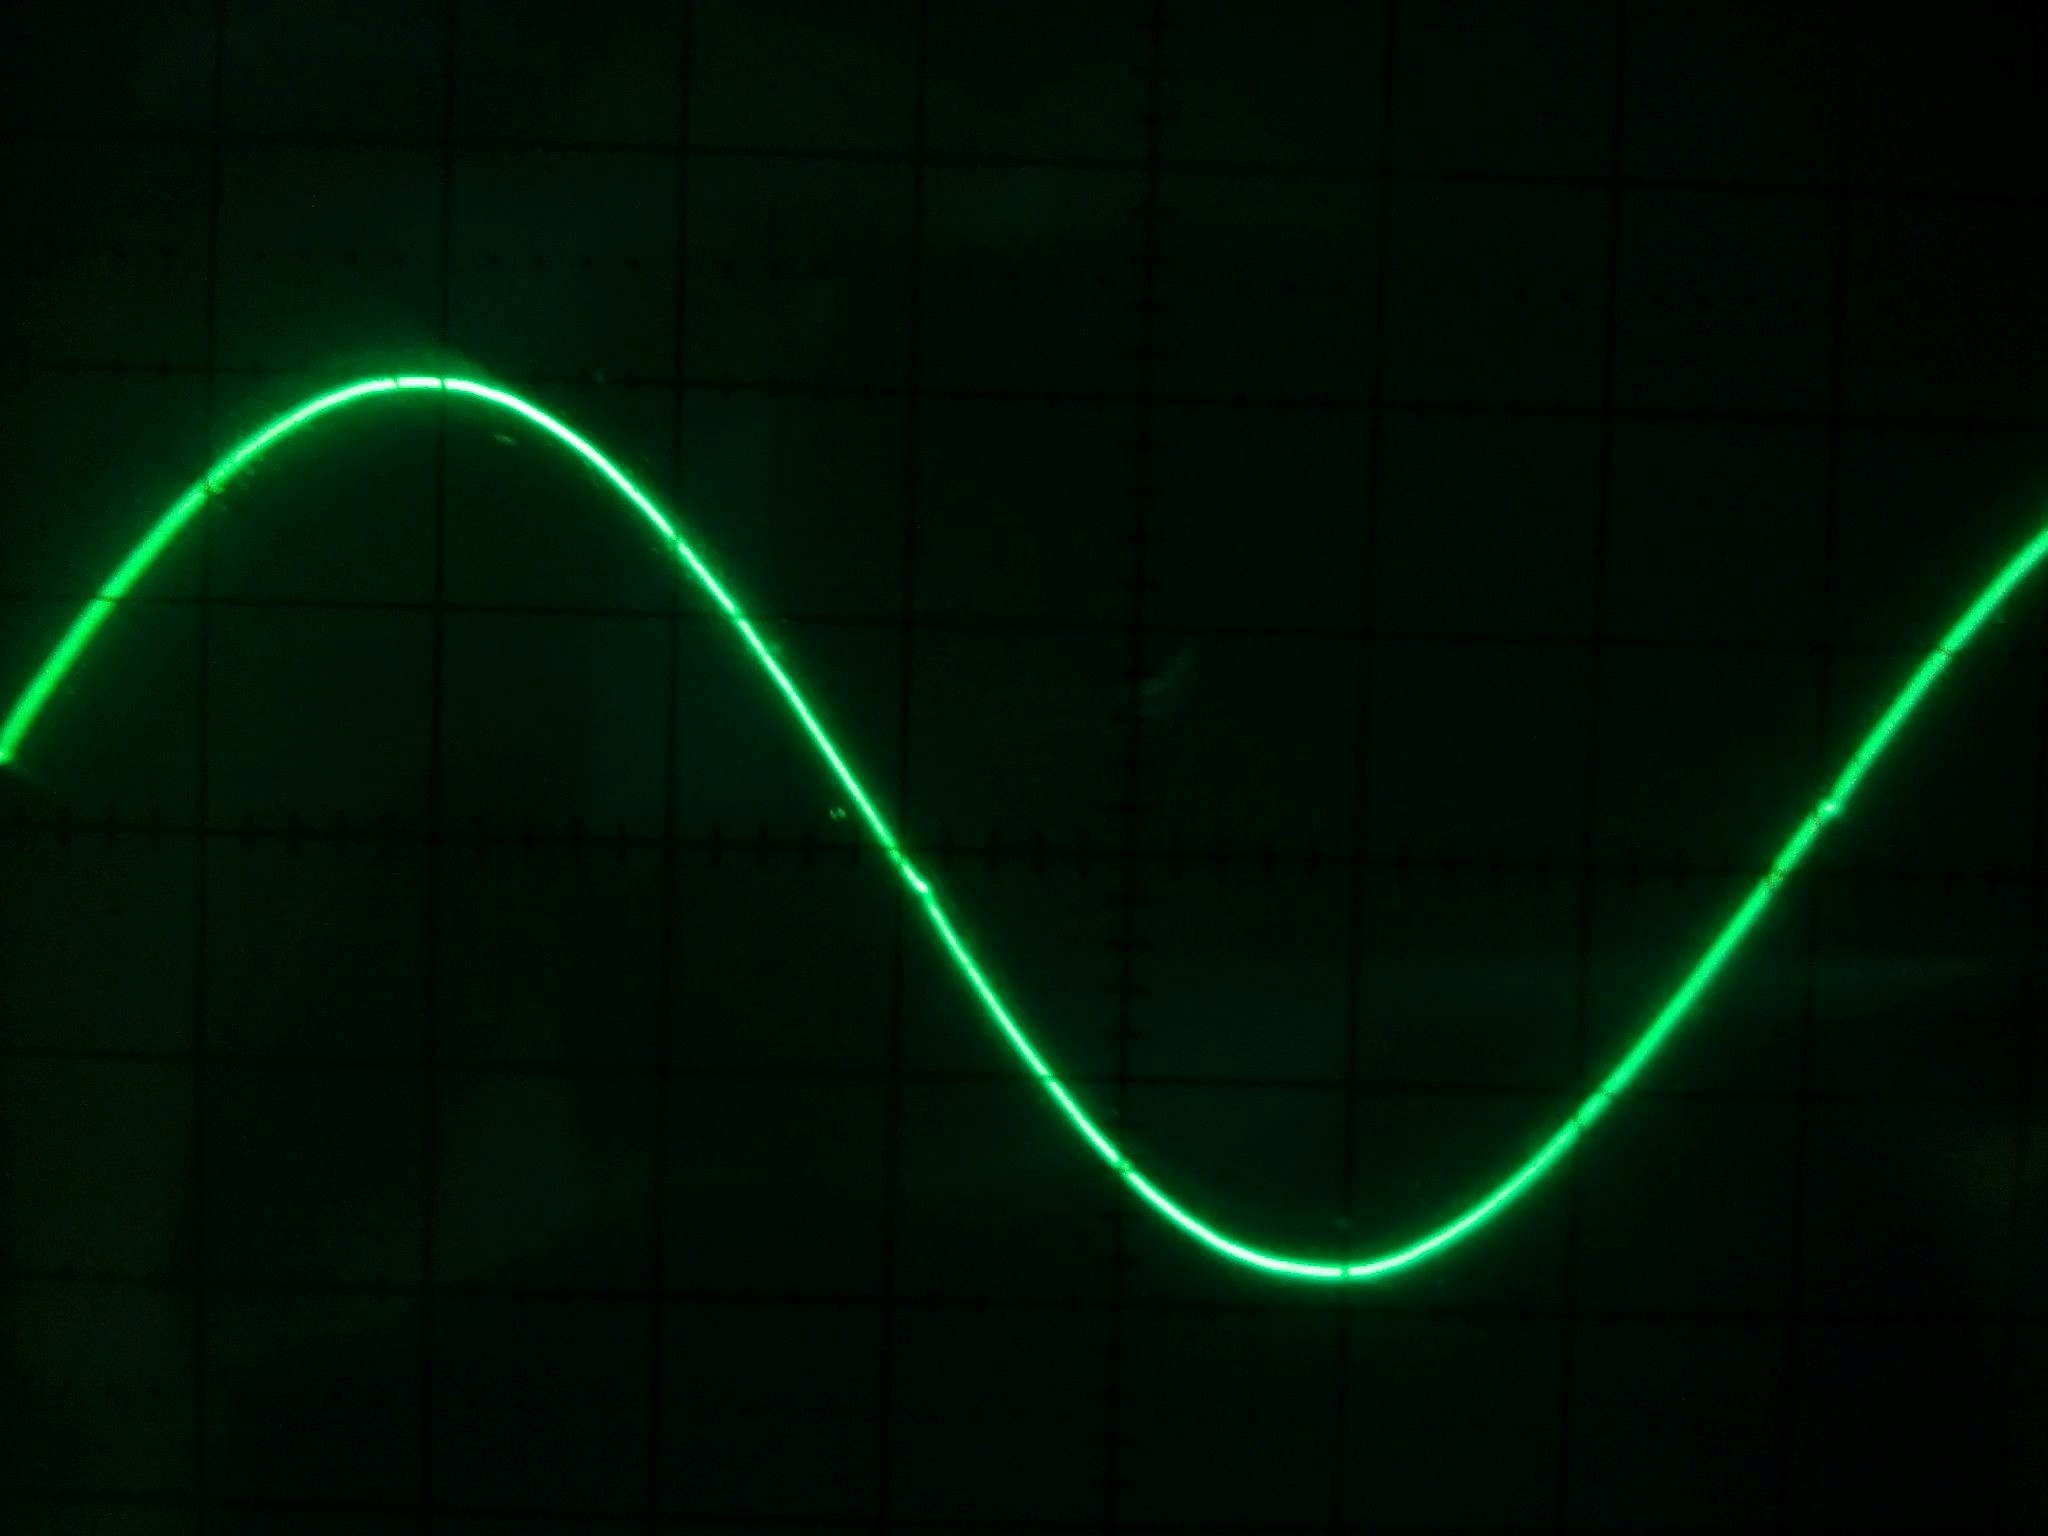
\includegraphics[width=0.8\textwidth]{pics/sinus-kurve}
      \end{center}
      \caption{Sinuskurve, Quelle: $\text{Computer:club}^2$, Urheber: Rolf Degen}
    \end{figure}
  \end{frame}

  \only<article>{Wir versuchen nun, mit Karos und unseren zwei Zuständen eine solche Kurve zu erzeugen. Nehmen wir an, dass ein ausgefülltes Karo dem Zustand ``AN'' entspricht, ein leeres Karo dem Zustand ``AUS''. Wenn man jetzt ausgefüllte Karos zu einer Pyramide zusammenstellt und dahinter an der Basis genau so eine Pyramide nach unten zeigen lässt, erhält man eine Annäherung an eine Sinuskurve.}

  \begin{frame}
  \framesubtitle{grobe Annäherung}
    \begin{center}
      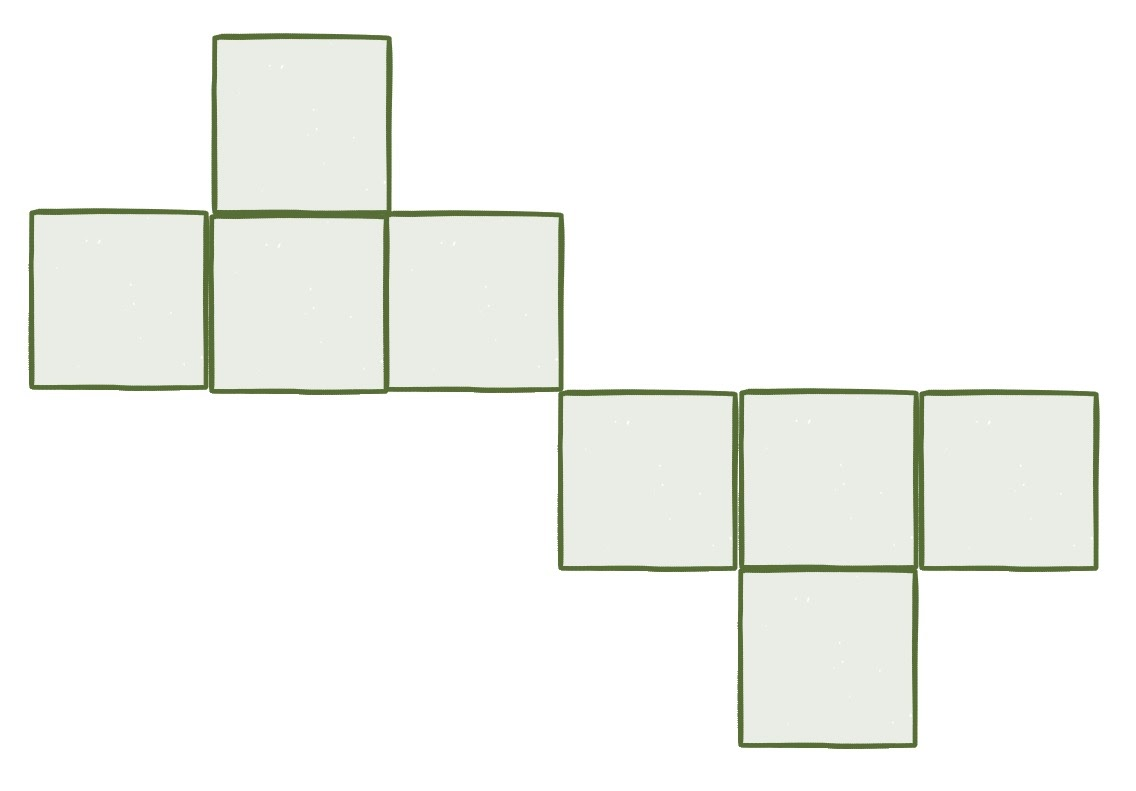
\includegraphics[width=0.8\textwidth]{pics/grobe-karos}
    \end{center}
  \end{frame}

  \only<article>{Je mehr Informationen wir verwenden, desto feiner wird die Annäherung an die Kurve.}

  \begin{frame}
  \framesubtitle{feinere Annäherung}
    \begin{center}  
      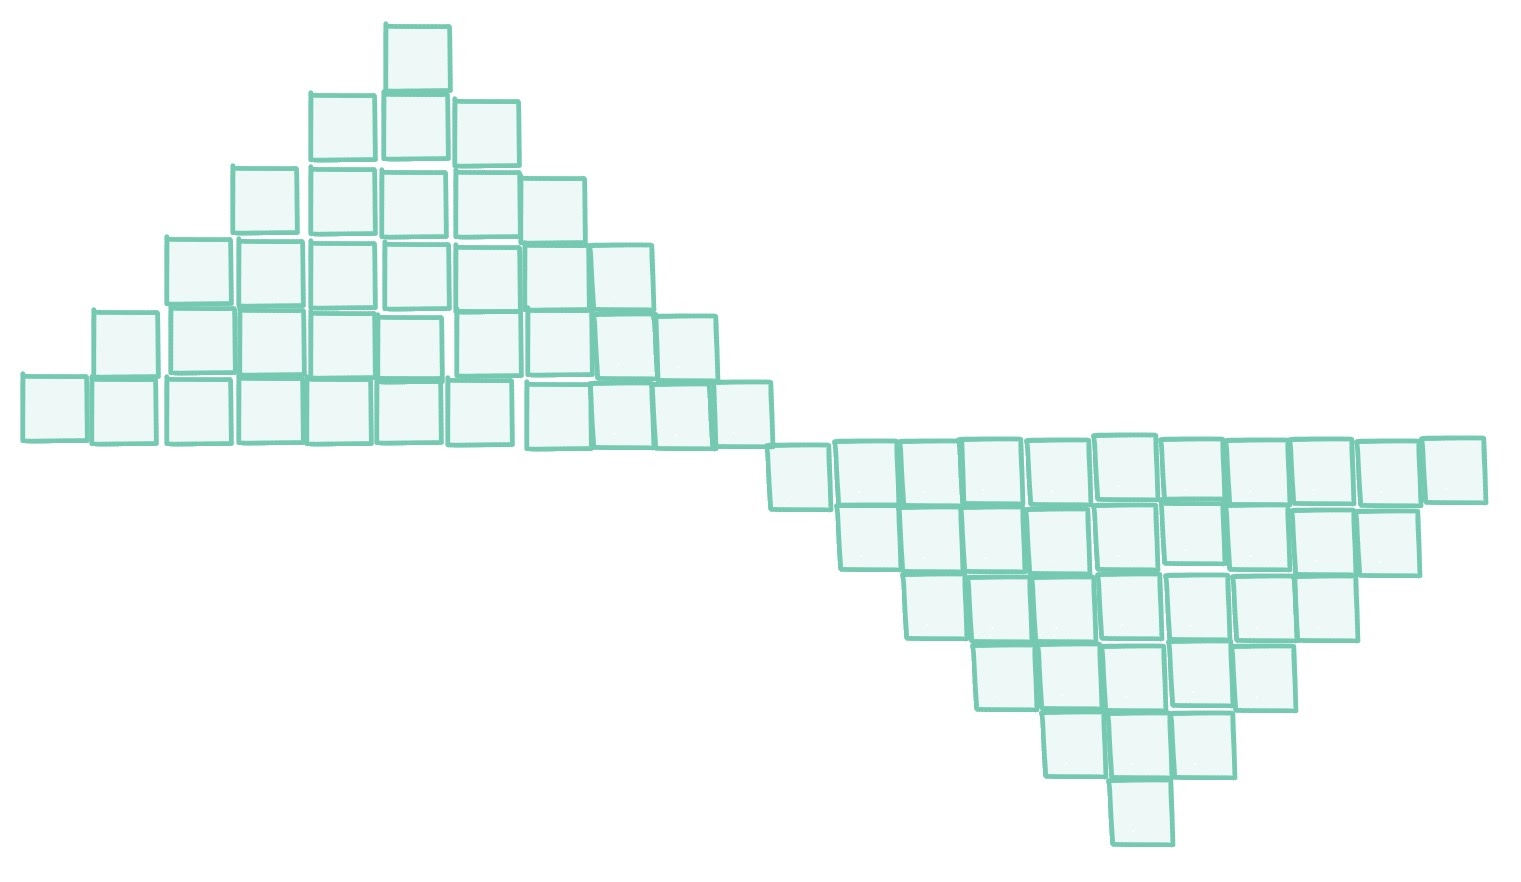
\includegraphics[width=0.8\textwidth]{pics/feine-karos}
    \end{center}
  \end{frame}

  \only<article>{Da unser Auge wie unser Ohr ein begrenzt feines Messinstrument ist, brauchen wir das Karo-Muster nur klein genug zu machen (oder weit genug weg zu nehmen) und können die Treppenstufen der Karos nicht mehr sehen bzw. hören.
  
    Mit ``AN'' / ``AUS'' Informationen lässt sich also die Wirklichkeit näherungsweise beschreiben.}

  \begin{frame}
    Je mehr ``an'' / ``aus'' Informationen wir einsetzen, desto näher ist das Ergebnis an der Wirklichkeit. Entsprechend steigen aber auch die benötigte Rechenleistung und der Speicherplatzbedarf an. 
  \end{frame}

  \begin{frame}
  \frametitle{Ein Bild mit wenig Informationen}
    \begin{figure}
      \begin{center}  
        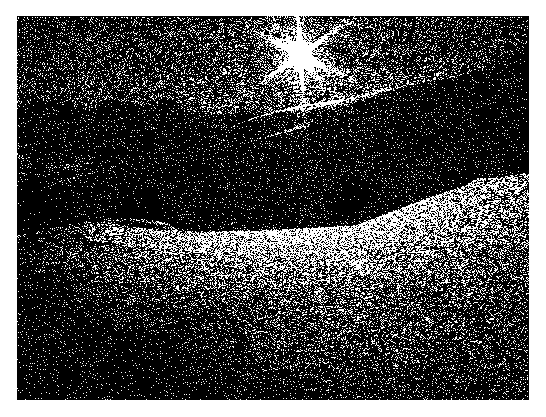
\includegraphics[width=0.8\textwidth]{pics/sw}
      \end{center}
    \end{figure}
  \end{frame}

  \begin{frame}
  \frametitle{Ein Bild mit vielen Informationen}
    \begin{figure}
      \begin{center}  
        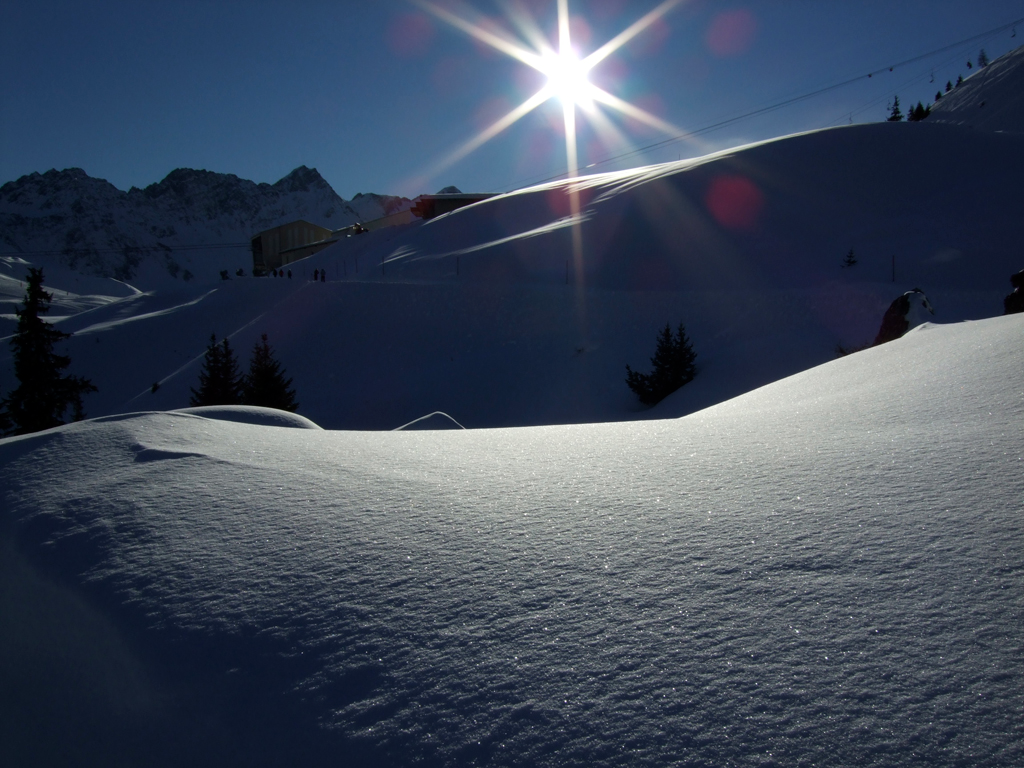
\includegraphics[width=0.8\textwidth]{pics/farbe}
      \end{center}
    \end{figure}
  \end{frame}

  \only<article>{Deshalb rechnet man mit speziellen Algorithmen ``nicht benötigte'' Informationen aus den Daten heraus.
  
    Auch wenn der Leistungszuwachs von Computern aussergewöhnlich ist, stehen Speicher und Rechenpower nicht unbegrenzt zur Verfügung und sollten ganz normal als Ressource wahrgenommen werden, die man nicht verschwendet.
  
    Übrigens: Zeitungspapier hält 10--50 Jahre, ein USB-Stick nur 3--10 Jahre. Für digitale Daten sind ausgeklügelte Backup-Systeme dringend notwendig!}
    


\section{Die Entwicklung des Internets}
  
  \begin{frame}
    \begin{figure}
      \begin{center}  
        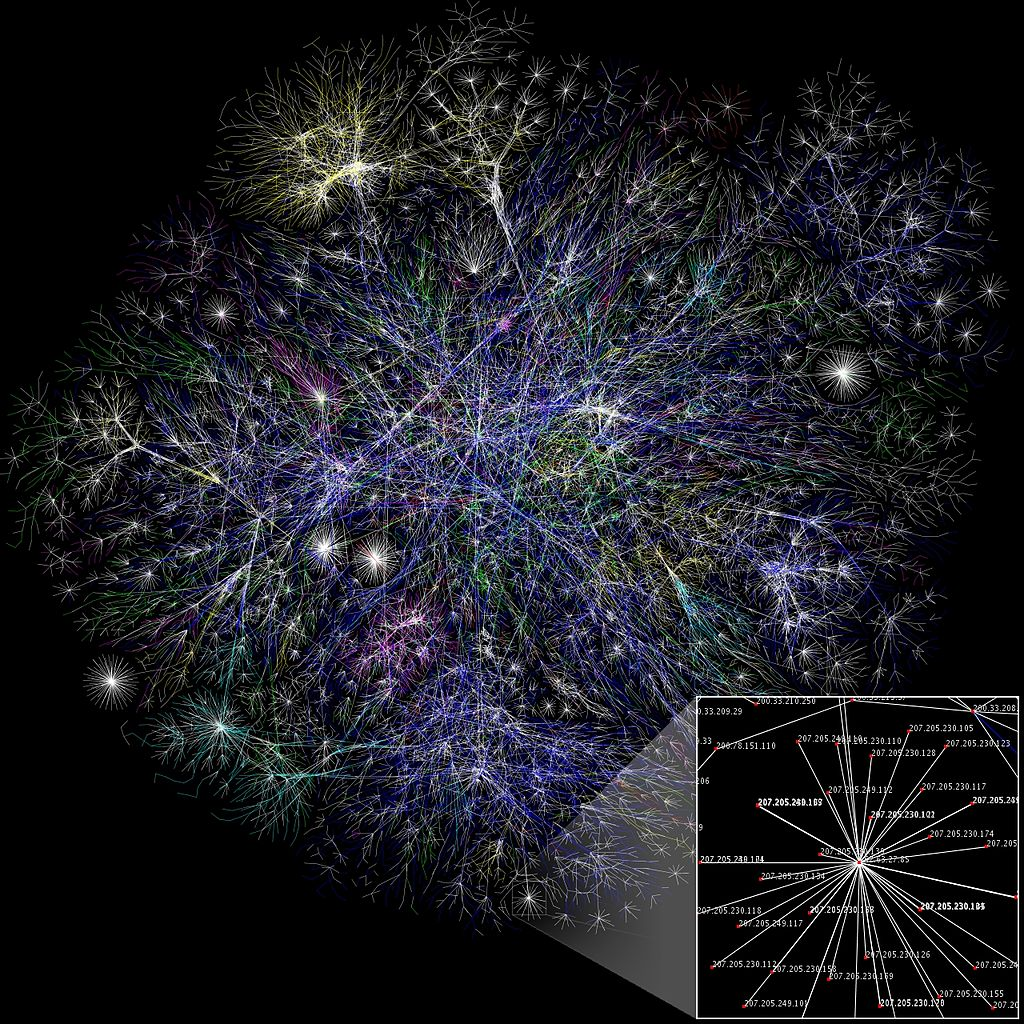
\includegraphics[width=0.6\textwidth]{pics/internet}
      \end{center}
      \pause
      \caption{Das Internet heute; Quelle: Wikipedia, Urheber: The Opte Project}
    \end{figure}
  \end{frame}

  \begin{frame}
    \frametitle<presentation>{Die Entwicklung des Internets}
    \framesubtitle{Meilensteine}
      \begin{itemize}
      \item ARPA
      \item E-Mail
      \item www --- ein neuer Treiber
      \item Web Apps, Cloud Services und intelligente Kühlschränke
    \end{itemize}
  \end{frame}

  \subsection{Der Vorläufer des Internets: Das Arpanet}
    \only<article>{
      Das Internet ist 1969 aus einer Zusammenarbeit des US--Verteidigungsministeriums und verschiedenen Forschungseinrichtungen entstanden. Obwohl sich das Gerücht hält, dass im kalten Krieg eine Technik aufgebaut werden sollte, die im Falle eines Atomschlages die Kommunikationsinfrastruktur erhalten kann, dürfte ein ausschlaggebender Grund für die Entwicklung die bessere Ausnutzung teurer Rechenkapazitäten gewesen sein. So entstand als Vorläufer des heutigen Internets das Arpanet.
    
      So oder so --- die Idee ist genial: Man teilt Kommunikation in kleine Päckchen auf und entwickelt Protokolle, die es ermöglichen, dass sich diese Päckchen ihren Weg selbständig vom Sender zum Empfänger suchen. Dabei gibt es nicht nur eine Leitung von A nach B, sondern ein fein verzweigtes Netzwerk mit unzähligen Knoten. Wenn nun eine Leitung blockiert ist, nimmt das Päckchen einfach einen anderen Weg.
    
      Übertragen wurden damals übrigens noch keine Webseiten mit Bildern.
    }

  \subsection{E-Mail}
    \only<article>{
      Beim Aufbau des Arpanet ging es um Kommunikation von Maschinen. Die Initiatoren konnten sich nicht vorstellen, dass der Austausch von Botschaften irgendeine Rolle in einem Netzwerk von wissenschaftlichen Computern spielen könnte. Aber schon Anfang der siebziger Jahre gab es Techniken, Nachrichten über das Netz auszutauschen, indem man dem Benutzernamen des Adressaten ein @ und den Namen des Computers anfügte.
    }

  \subsection{www : am CERN wird Internet--Geschichte geschrieben}
    \only<article>{
      Das CERN spielt eine wichtige Rolle bei der Entwicklung des Internets, wie wir es heute kennen. Die Laboratorien des CERN liegen teilweise auf schweizer Gebiet, teilweise auf französischem. Natürlich setzt jedes Land seine eigenen Systeme ein, was es damals unmöglich machte, Texte online auszutauschen.
    
      Mitte der achtziger Jahre nahm sich ein britischer Physiker und Informatiker namens Tim Berners--Lee dieses Problems an und entwickelt mit seinem Kollegen Robert Cailliau ein Konzept für ein weltweites Hypertext--Projekt, das sie 1990 veröffentlichen. Das daraus entstehende Protokoll ``http'' und die Auszeichnungsprache ``html'' sind auch heute noch die Grundlagen des \textbf{W}orld\textbf{W}ide\textbf{W}eb. Dabei geht es darum Texte über das Netzwerk zur Verfügung stellen zu können.
    
      Die Problematik, Texte universell für verschiedenste System darstellbar zu übertragen, wird auch heute noch deutlich, wenn man z.B. eine Webseite auf einem Smartphone öffnet, die für den Desktop optimiert ist.
    
      Inzwischen sind die Texte um Bilder ``bereichert'', Filme werden über das Internet gestreamt und Weltkarten in 3D betrachtet.
      Sag‘ bloss... kann ich hiermit tippen?
    }

  \subsection{Internet der Dinge}
    \only<article>{
      Da man nun immer mehr Leistung in immer kleinere Chips packen kann, können kleinste Dinge Funktionen bekommen, für die man früher ganze Rechenzentren benötigte.
    
      Wecker zeigen das Wetter an, Kalender berechnen die Wegzeit automatisch in Alarme mit ein, Navigationssysteme verwenden aktuelle und zu erwartende Verkehrsdaten, um die optimale Route zu bestimmen. Für all das benötigen die Dinge eine Verbindung zum Internet.
    
      Das wirft verschiedene Probleme auf: Sicherheit und Datenschutz sind ein Thema. Aber auch technisch braucht es neue Ansätze. So muss jeder, der an ihn gerichtete Informationen bekommen will, eindeutig identifizierbar sein. Die ursprünglich für diesen Zweck gemachte Adressierung (IPv4) hat für das Internet der Dinge viel zu wenig Adressen. Eine neue Technik zur Adressierung ist vorhanden, setzt sich aber nur langsam durch.}


\section{Server}
  \begin{frame}
      \frametitle<presentation>{Server}
      \begin{itemize}
        \item Hardware
        \item Virtualisierung
       \item Software
    \end{itemize}
  \end{frame}
    
  \subsection{Hardware}
    \begin{frame}
      \begin{figure}
      \begin{center}  
        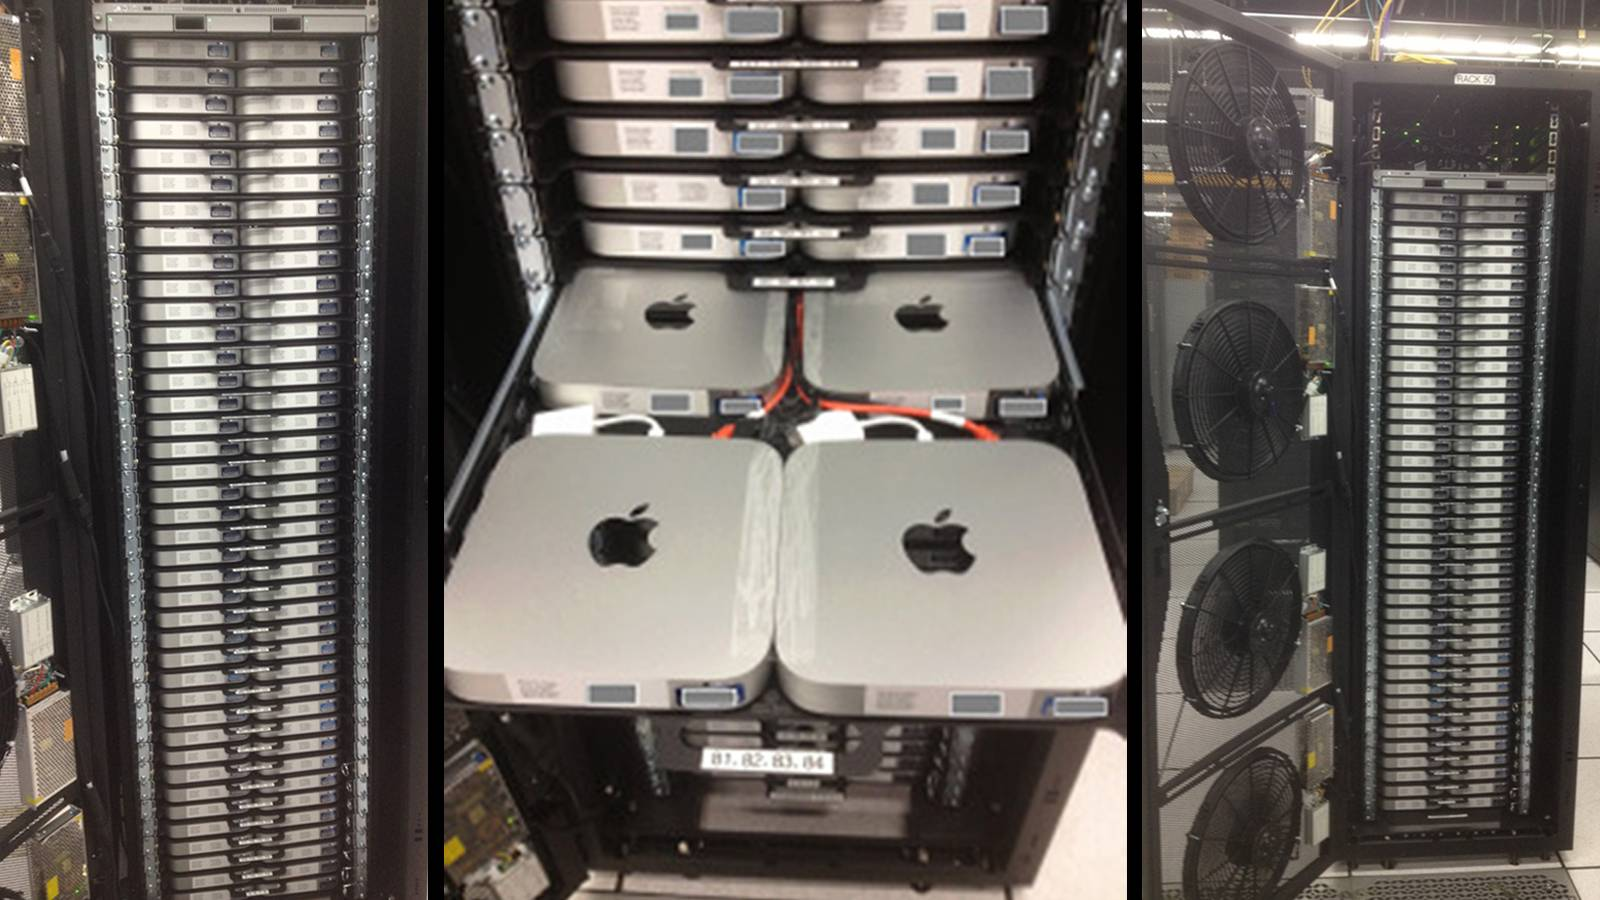
\includegraphics[width=1\textwidth]{pics/MacMiniServer}
      \end{center}
      \caption{MacMini Server; Quelle: Gizmodo India}
    \end{figure}
    \end{frame}
      
      \only<article>{Was ist ein Server? Im Grunde genommen ist jedes Gerät, das Dienstleistungen zur Verfügung stellt, ein Server. Wenn ich von meinem lokalen PC eine Webseite bereit stelle, die jemand anderes von seinem PC aufruft, ist mein PC in dem Moment ein Server.
      
            Ursprünglich war Rechenleistung so teuer, dass es nur einen riesigen Rechner in einem gut gekühlten Keller gab. Terminals ohne eigene Rechenkapazität stellten für eine Anzahl von Nutzern eine Verbindung zu diesem Rechner her, dessen Leistung unter allen Nutzern aufgeteilt wurde. Irgendwann wurde die Technik so billig, dass mit dem Aufkommen der Personal Computers jeder seinen eigenen Rechner auf seinem Schreibtisch hatte. 
      
            Das Moorsche Gesetz besagt dass sich die Rechenleistung alle (je nach Quelle) ein bis zwei Jahre verdoppelt.
      
            Inzwischen haben wir mehr Leistung in einem Mobiltelefon, als noch vor zehn Jahren auf dem Desktop.
      
            Im Jahr 2000 wurden für den Aufbau einer Datenbank für kurze Texte noch 40.000 DM für einen Server der Firma SUN ausgegeben. Der Vorschlag, stattdessen einen Linux--PC für 5.000 DM einzusetzen war revolutionär\ldots\ und erfolgreich. Tatsächlich waren die PCs so leistungsfähig geworden, dass es keinen Grund mehr gab, das Achtfache zu investieren.
      
            Sogar MacMinis wurden schon benutzt, um den kompletten Webauftritt von Firmen zu realisieren.}

    \subsection{Virtualisierung}
    \begin{frame}
      \frametitle<presentation>{Virtualisierung}
        \begin{figure}
          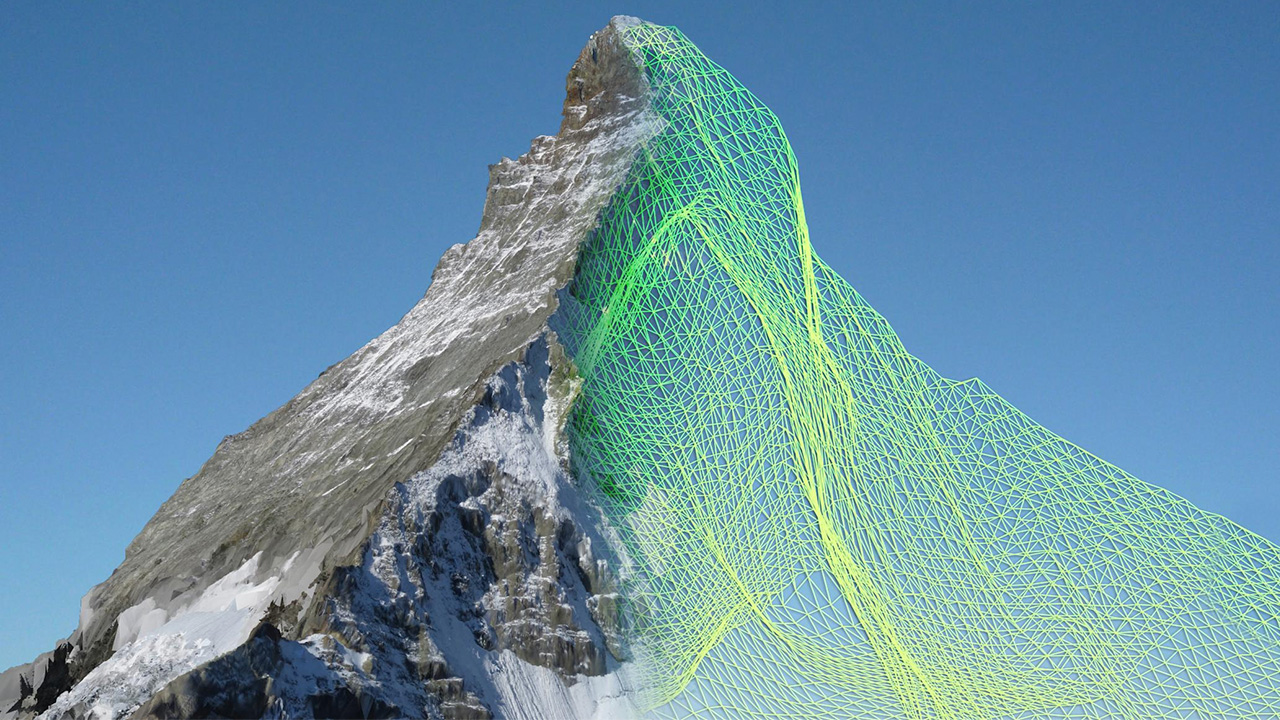
\includegraphics[width=1\textwidth]{pics/Matterhorn}
          \caption{Photomontage: Jamani Caillet / © EPFL\newline
          \hspace{\linewidth}http://actu.epfl.ch/news/the-matterhorn-like-you-ve-never-seen-it/}
        \end{figure}
    \end{frame}
      
      \only<article>{Hardware ist so billig --- warum sollte man einen PC virtualisieren wollen?
      
            Seit Microsoft mit seinen Produkten den PC--Markt beherrscht, stellt sich für Nicht--Windows--Nutzer das Problem, wie man Word--Dokumente öffnen soll. Man glaubt es kaum, aber es gab und gibt immer noch Menschen, die kein Word haben; oder es schlicht nicht benutzen wollen. Aber auch diese Leute bekommen regelmässig Anhänge mit der berühmten Endung ``.docx''. Auch gibt es viel Software, die ausschliesslich für Windows geschrieben wurde. 
      
            Schliesslich hatte ein PC genug Leistung für zwei, und so sind kluge Köpfe auf die Idee gekommen, einen PC innerhalb eines PCs zu simulieren. Was bedeutet das? Um diese Frage zu klären, müssen wir uns erstmal bewusst werden, was ein PC ist.}

      \begin{frame}
        \frametitle{die Komponenten eines PCs}
        \begin{figure}
          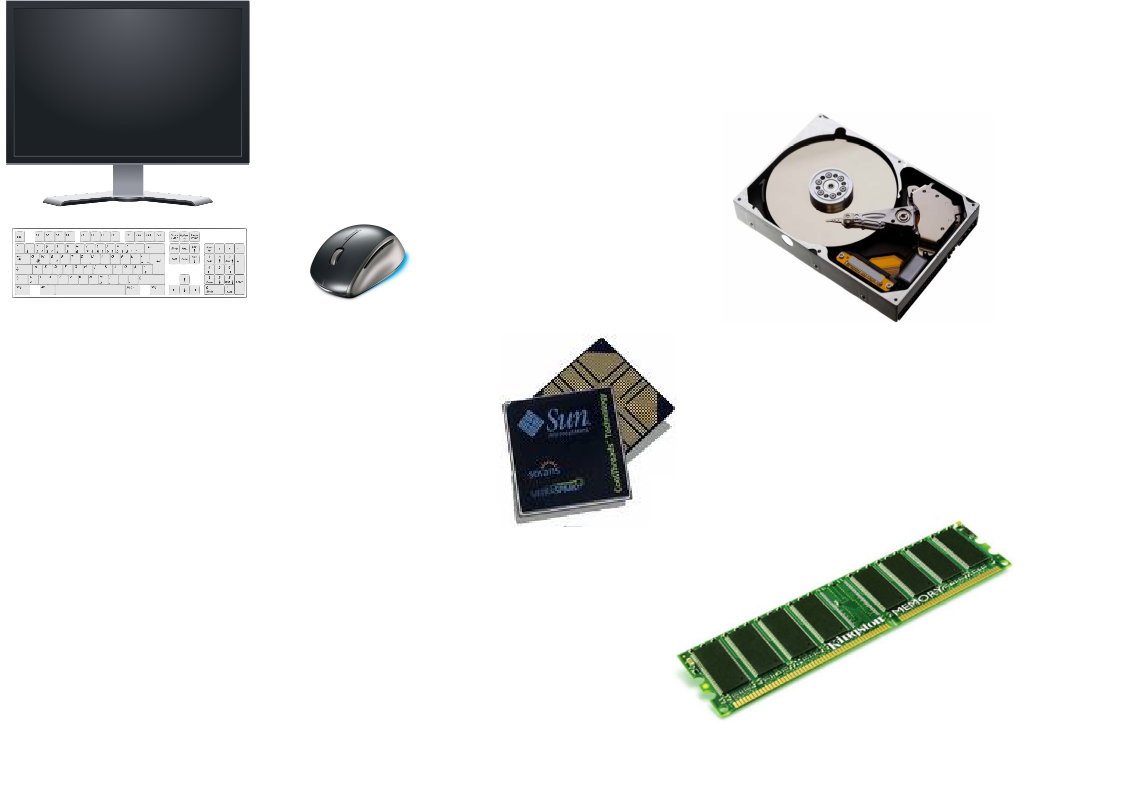
\includegraphics[width=1\textwidth]{pics/pc-komponenten}
        \end{figure}
      \end{frame}

      \only<article>{Das Herzstück des PCs ist der Prozessor --- der eigentliche Rechner. 
      
            Damit man mit ihm kommunizieren kann, gibt es Ein-- und Ausgabesysteme. Bis in die achtziger Jahre wurden dafür z.B. Lochkarten gebraucht, heute benutzen wir im Wesentlichen Tastatur und Maus, immer öfter auch den Touchscreen. Monitore und Drucker sind Beispiele für Ausgabesysteme.
      
            Die Daten müssen irgendwo gespeichert werden. Auch hierfür taugt die Lochkarte bzw. ganze Lochbänder, inzwischen abgelöst durch magnetische Medien, optische Datenträger und nichtflüchtige elektronische Speicher.
      
            ``Nichtflüchtig'' leitet zu einem weiteren Speicher über: Der Prozessor eines PCs ist so schnell, dass er einen besonderen, schnellen Zwischenspeicher benötigt, von dem er Daten laden und auf dem er seine Ergebnisse ablegen kann. Die Rede ist vom RAM, ein schneller elektronischer Speicher, der allerdings seine Informationen sofort verliert, wenn der Strom abgeschaltet wird.
      
            Auf den meisten Heim--PCs ist heutzutage nicht mehr der Prozessor (CPU) der schnellste im Team. Den Titel hat er an den Grafikprozessor (GPU) abgegeben. Dazu muss man wissen, dass die Spieleentwicklung einer der Treiber bei der technischen Entwicklung von PCs ist. Und für Bilder gilt genauso wie für alles Digitalisierte: Je wirklichkeitsgetreuer die Darstellung sein soll, desto mehr ``AN'' / ``AUS'' Informationen brauchen wir, und desto leistungsfähiger muss die Hardware sein.
      
            Verbunden werden all die Komponenten durch das sogenannte Motherboard. Auf ihm sitzt auch ein weiterer kleiner Chip, der beim Einschalten des PCs erstmal die Komponenten sortiert und entscheidet, was gestartet werden soll. Das Problem ist nämlich, dass kein Bauteil vom anderen ``weiss''. Wir brauchen eine Software, die die Bauteile miteinander verknüpft, das Betriebssystem. Das Betriebssystem übernimmt vom Chip die Hoheit über den Computer und stellt uns unsere Arbeitsumgebung --- im Alltag also den Desktop mit Mail--Programm, Textverarbeitung usw. --- zur Verfügung.
      
            Der Clou ist, dass man alle diese Komponenten entweder teilen oder komplett simulieren kann. Wenn ein PC beispielsweise 8GB RAM hat, dann kann man 4GB davon für einen virtuellen PC benutzen. Unserem PC, unserem Betriebssystem stehen dann nur noch 4GB zur Verfügung, die übrigen 4GB ``gehören'' der virtuellen Maschine.
      
            Man startet also seinen PC, meldet sich an und ruft ein Programm auf, das per Software nun alle Komponenten eines PCs noch einmal simuliert und diesen virtuellen PC startet. Eine Festplatte in diesem ``PC'' ist dann nur eine grosse Datei auf unserer echten Festplatte. Und in diesem virtuellen PC lässt sich dann ein eigenes Betriebssystem installieren. Auf diesem Weg hat man nun auf einem PC gleichzeitig Windows und Linux zur Verfügung.
      
            Da die Leistungsfähigkeit der Hardware inzwischen so stark gestiegen ist, kann man auf einem Computer gleichzeitig mehrere virtuelle PCs starten.}
      
      \begin{frame}
      \frametitle{Vorteile der Virtualisierung}
        \begin{itemize}
          \item Da virtuelle Computer nur Dateien auf einer Festplatte sind, kann man sie komplett in einem Backup sichern und quasi auf Knopfdruck wieder herstellen.
          \item Wenn man für einen Computer kurzfristig mehr Leistung braucht, kann man einem virtuellen Computer einfach per Software mehr RAM oder weitere CPUs zur Verfügung stellen. Das geht teilweise unterbruchsfrei.
          \item Computer sind selten ausgelastet. Wenn man seinen Bedarf auf virtuelle Maschinen verteilt, ist die Auslastung der echten Systeme besser.
        \end{itemize}
      \end{frame}

    \subsection{Software}

      \only<article>{Das Wort Server wird synonym auch für die Software benutzt, die dafür zuständig ist, Services zu erbringen. Wenn wir von einem Webserver sprechen, kann sowohl die (virtuelle) Maschine gemeint sein, die die Webseiten ausliefert, als auch die Software auf der Maschine, die diese Arbeit übernimmt.}

      \begin{frame}
      \frametitle{Beispiele für Software--Server}
        \begin{itemize}
          \item Webserver
          \item Mailserver
          \item Dateiserver
          \item Datenbankserver
        \end{itemize}
      \end{frame}

      \only<article>{Immer übernimmt eine entsprechende Software die Aufgabe, Daten auszuliefern bzw. zu empfangen. Auf einem Hardwareserver können mehrere Softwareserver laufen, auch wenn es im Zuge der Virtualisierung sinnvoll erscheint, für jeden Serverzweck eine eigene virtuelle Maschine zu Verfügung zu stellen. So läuft in der ETH--Bibliothek z.B. das Bibliothekssystem auf einem Server, die Datenbank auf einem anderen.}
  
  